\paragraph{}Da bi bila aplikacija "cim bolj prijazna uporabniku je "sla "cez veliko razli"cic in popravkov. V nadaljevanju je opisano kako deluje trenutno najnovej"sa razli"cica 3.0. Izvorna koda je dostopna na spletnem portalu GitHub na naslovu \url{https://github.com/GimVic-app/gimvic-ios}.

\subsection{Podatki} 
\paragraph{}Podatki, ki jih aplikacija potrebuje, so servirani iz razli"cnih stre"znikov v razli"cnih oblikah zapisa. Urnik je na voljo v JavaScript array obliki, nadome"s"canja pa v json. Jedilnik za "solsko malico in kosilo se nalo"zi na stre"znik v csv obliki. Odlo"cil sem se, da bo za podatke skrbel poseben stre"znik, ki bo vse od zgoraj na"stetega zdru"zil v enovito json obliko, ker bo tako prikazovanje na telefonu hitrej"se in bolj u"cinkovito. Podatki na tem stre"zniku so na voljo v json obliki.

\paragraph{}Pri dostopu do podatkov stre"zniku poda"s ali "zeli"s podatke za profesorja, ali pa za dijaka. Pri profesorju stre"zniku kot parameter poda"s ime profesorja, pri dijaku pa razred in izbirne ozroma maturitetne predmete. Stre"znik nato vrne seznam, kjer vsak element v tem seznamu predstavlaj podatke za dolo"cen dan v tednu. Vsak dan je predstavljen z seznamom v katerem vsak element predstavlja uro.

\newpage
\subsection{Sestava aplikacije}
Aplikacija je sestavljena iz dveh glavnih delov:
\begin{itemize}
	\setlength\itemsep{0em}
	\item glavna aktivnost (\textit{ang.} root view controller)
	\item upravitelj podatkov
	\item nastavitve
	\item o aplikaciji
\end{itemize}

\subsubsection{Glavna aktivnost}
\begin{wrapfigure}{r}{0.4\linewidth}
	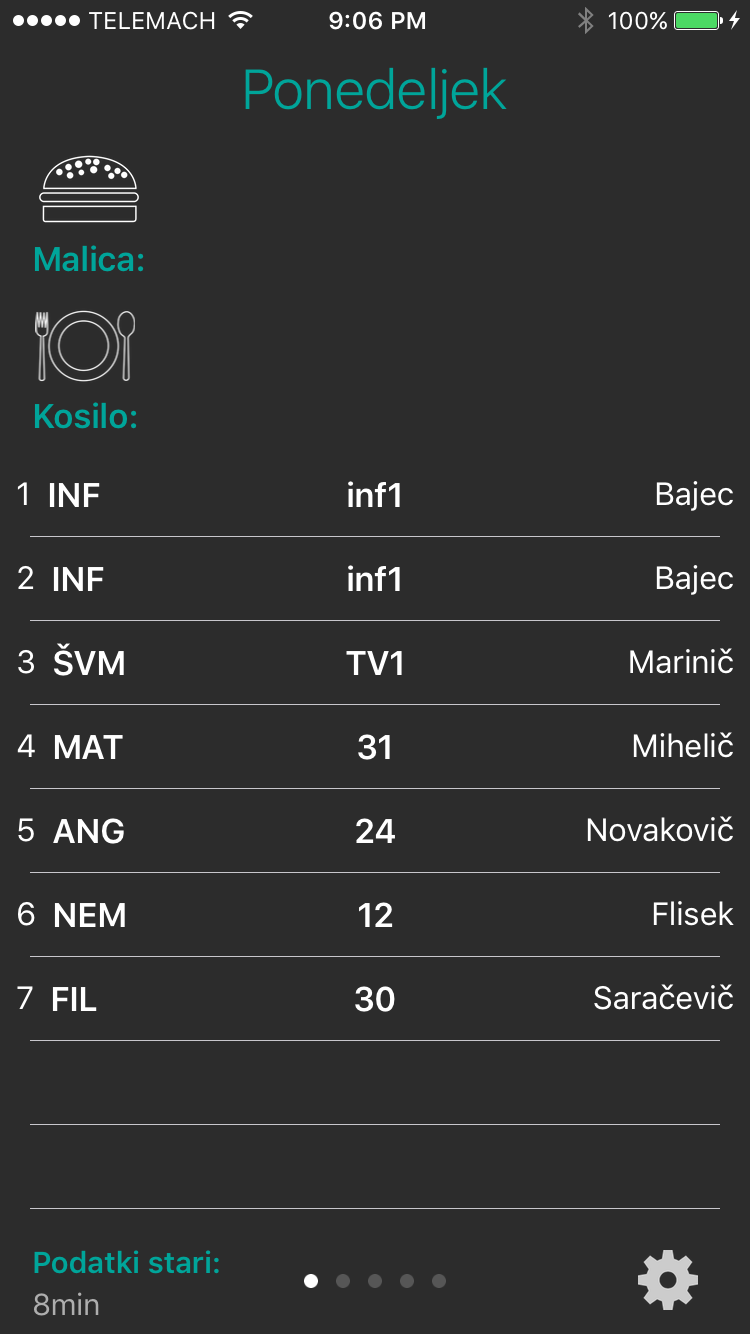
\includegraphics[width=\linewidth]{images/main_view.png}
\end{wrapfigure}
\paragraph{}Tu se odvija ve"cino uporabniku pomembnih stvari. Ko uporabnik odpre aplikacijo se mu prika"ze glavni pogled (\textit{ang.} main view) v katerem je za vsak dan prikazan jedilnik in urnik. V glavni aktivnosti se nahaja tudi gumb za nastavitve.

\paragraph{}Ko se glavna aktvinost odpre, aplikacija najprej preveri, "ce je odprta prvi"c. V tem primeru uporabniku prika"ze navodila za uprabo in ga popelje "cez osnovne nastavitve kjer nastavi razred oziroma ime profesorja, ter vrsto malice in kosila.

\subsubsection{Upravitelj podatkov}
\paragraph{}Upravitelj podatkov skrbi za pridobivanje podatkov iz stre"znika, njihovo obdelovanje in shranjevanje. Za"zene se vsaki"c ko se aplikacija odpre in najprej preveri starost trenutno shranjenih podatkov. "Ce so podatki prestari gre na stre"znik po nove podatke, ki jih pretvori v primerne podatkovne strukture in shrani na pomnilnik telefona. Nato o novih podatkih obvesti glavno aktivnost, ki osve"zi grafi"cni vmesnik z novimi podatki.

\paragraph{}"Ce upravitelj podatkov ugotovi, da naprava nima internetne povezave uporabi podatke, ki so "ze shranjeni na napravi. Uporabnik lahko podatke osve"zi ro"cno. V tem primeru glavna aktivnost zahteva od upravitelja podatkov, da gre po nove podatke.

\subsubsection{Nastavitve}
\begin{wrapfigure}{r}{0.4\linewidth}
	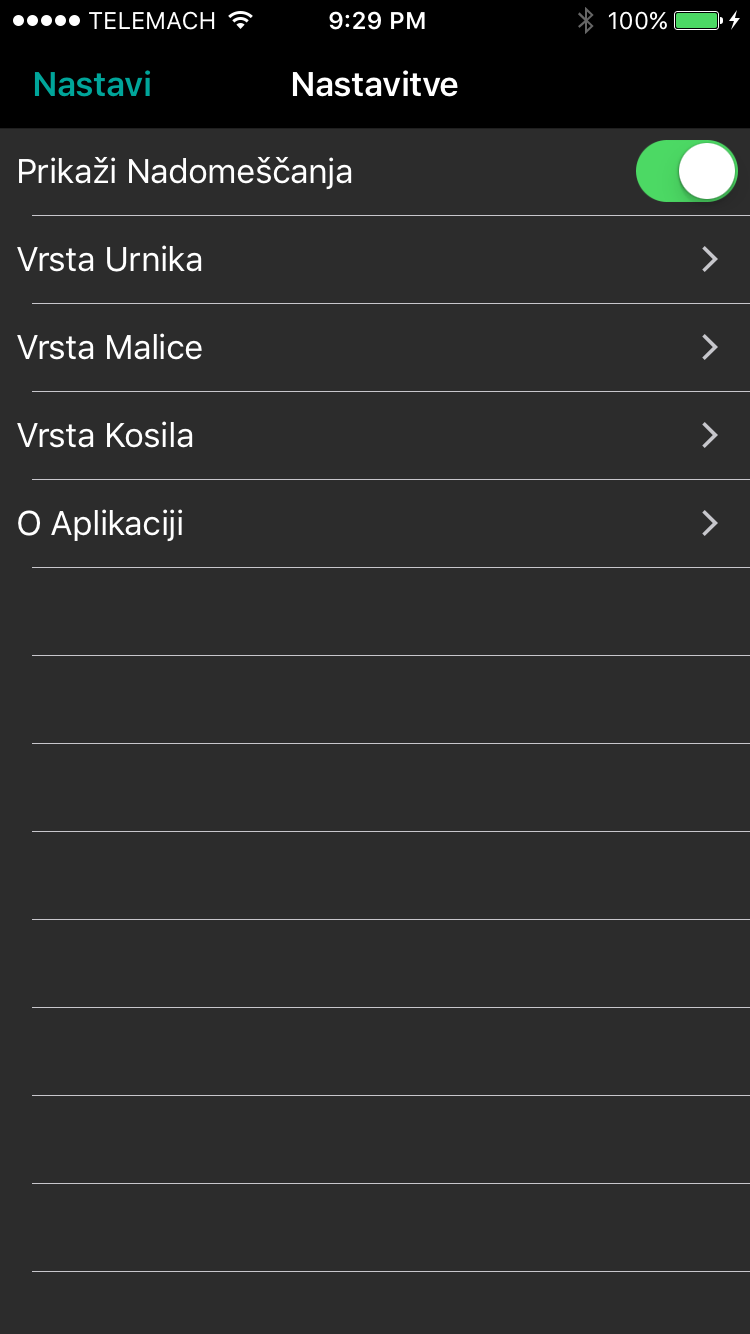
\includegraphics[width=\linewidth]{images/nastavitve.png}
\end{wrapfigure}
\paragraph{}V nastavitvah lahko uprabnik nastavi ali je dijak, ali profesor in temu primeren filter za urnik. Nastavi lahko tudi vrsto malice in kosila na katerega je naro"cen. Poleg tega ima tudi mo"znost, da izklopi funkcijo za prikaz nadome"s"canj, tako da je uporabniku prikazan samo urnik. V nastavitvah lahko uporabnik pogleda podatke o aplikaciji.

\subsubsection{O aplikaciji}
\paragraph{}V tem meniju se uporabniku prika"zejo osnovne informacije o aplikaciji kot so avtor aplikacije, verzija in pod katero licenco je aplikacija izdana. Prav tako je v tem meniju zapisan vir nekaterih ikon, ki so uporabljene, saj to predpisuje licenca pod katero so izdane te ikone.
